\documentclass{standalone}
\usepackage{xcolor}
\usepackage{tikz}
\usepackage{pgfplots}
\usepackage{pgfplots}
\usepgfplotslibrary{colormaps}
\pgfplotsset{compat=1.16}
\usetikzlibrary{positioning, backgrounds}

\input{figures/colmaps}

\begin{document}


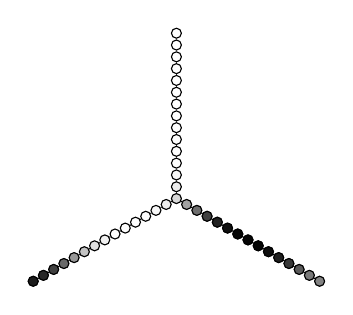
\begin{tikzpicture}[scale=.3]

\draw[color=black,thin] (0.000000,0.000000)--(0.000000,0.500000);
\draw[color=black,thin] (0.000000,0.500000)--(0.000000,1.000000);
\draw[color=black,thin] (0.000000,1.000000)--(0.000000,1.500000);
\draw[color=black,thin] (0.000000,1.500000)--(0.000000,2.000000);
\draw[color=black,thin] (0.000000,2.000000)--(0.000000,2.500000);
\draw[color=black,thin] (0.000000,2.500000)--(0.000000,3.000000);
\draw[color=black,thin] (0.000000,3.000000)--(0.000000,3.500000);
\draw[color=black,thin] (0.000000,3.500000)--(0.000000,4.000000);
\draw[color=black,thin] (0.000000,4.000000)--(0.000000,4.500000);
\draw[color=black,thin] (0.000000,4.500000)--(0.000000,5.000000);
\draw[color=black,thin] (0.000000,5.000000)--(0.000000,5.500000);
\draw[color=black,thin] (0.000000,5.500000)--(0.000000,6.000000);
\draw[color=black,thin] (0.000000,6.000000)--(0.000000,6.500000);
\draw[color=black,thin] (0.000000,6.500000)--(0.000000,7.000000);

\draw[color=black,thin] (0.000000,0.000000)--(-0.433013,-0.250000);
\draw[color=black,thin] (-0.433013,-0.250000)--(-0.866025,-0.500000);
\draw[color=black,thin] (-0.866025,-0.500000)--(-1.299038,-0.750000);
\draw[color=black,thin] (-1.299038,-0.750000)--(-1.732051,-1.000000);
\draw[color=black,thin] (-1.732051,-1.000000)--(-2.165064,-1.250000);
\draw[color=black,thin] (-2.165064,-1.250000)--(-2.598076,-1.500000);
\draw[color=black,thin] (-2.598076,-1.500000)--(-3.031089,-1.750000);
\draw[color=black,thin] (-3.031089,-1.750000)--(-3.464102,-2.000000);
\draw[color=black,thin] (-3.464102,-2.000000)--(-3.897114,-2.250000);
\draw[color=black,thin] (-3.897114,-2.250000)--(-4.330127,-2.500000);
\draw[color=black,thin] (-4.330127,-2.500000)--(-4.763140,-2.750000);
\draw[color=black,thin] (-4.763140,-2.750000)--(-5.196152,-3.000000);
\draw[color=black,thin] (-5.196152,-3.000000)--(-5.629165,-3.250000);
\draw[color=black,thin] (-5.629165,-3.250000)--(-6.062178,-3.500000);


\draw[color=black,thin] (0.000000,0.000000)--(0.433013,-0.250000);
\draw[color=black,thin] (0.433013,-0.250000)--(0.866025,-0.500000);
\draw[color=black,thin] (0.866025,-0.500000)--(1.299038,-0.750000);
\draw[color=black,thin] (1.299038,-0.750000)--(1.732051,-1.000000);
\draw[color=black,thin] (1.732051,-1.000000)--(2.165064,-1.250000);
\draw[color=black,thin] (2.165064,-1.250000)--(2.598076,-1.500000);
\draw[color=black,thin] (2.598076,-1.500000)--(3.031089,-1.750000);
\draw[color=black,thin] (3.031089,-1.750000)--(3.464102,-2.000000);
\draw[color=black,thin] (3.464102,-2.000000)--(3.897114,-2.250000);
\draw[color=black,thin] (3.897114,-2.250000)--(4.330127,-2.500000);
\draw[color=black,thin] (4.330127,-2.500000)--(4.763140,-2.750000);
\draw[color=black,thin] (4.763140,-2.750000)--(5.196152,-3.000000);
\draw[color=black,thin] (5.196152,-3.000000)--(5.629165,-3.250000);
\draw[color=black,thin] (5.629165,-3.250000)--(6.062178,-3.500000);




%0 of colormap/blackwhite}

\filldraw[color of colormap={920 of colormap/blackwhite}] (0.000000,0.500000) circle (6.0pt);

\filldraw[color of colormap={960 of colormap/blackwhite}] (0.000000,1.000000) circle (6.0pt);

\filldraw[color of colormap={990 of colormap/blackwhite}] (0.000000,1.500000) circle (6.0pt);
\filldraw[color of colormap={990 of colormap/blackwhite}] (0.000000,2.000000) circle (6.0pt);
\filldraw[color of colormap={1000 of colormap/blackwhite}] (0.000000,2.500000) circle (6.0pt);
\filldraw[color of colormap={1000 of colormap/blackwhite}] (0.000000,3.000000) circle (6.0pt);
\filldraw[color of colormap={1000 of colormap/blackwhite}] (0.000000,3.500000) circle (6.0pt);
\filldraw[color of colormap={1000 of colormap/blackwhite}] (0.000000,4.000000) circle (6.0pt);
\filldraw[color of colormap={1000 of colormap/blackwhite}] (0.000000,4.500000) circle (6.0pt);
\filldraw[color of colormap={1000 of colormap/blackwhite}] (0.000000,5.000000) circle (6.0pt);
\filldraw[color of colormap={1000 of colormap/blackwhite}] (0.000000,5.500000) circle (6.0pt);
\filldraw[color of colormap={1000 of colormap/blackwhite}] (0.000000,6.000000) circle (6.0pt);
\filldraw[color of colormap={1000 of colormap/blackwhite}] (0.000000,6.500000) circle (6.0pt);
\filldraw[color of colormap={1000 of colormap/blackwhite}] (0.000000,7.000000) circle (6.0pt);

\filldraw[color of colormap={630 of colormap/blackwhite}] (0.433013,-0.250000) circle (6.0pt);
\filldraw[color of colormap={430 of colormap/blackwhite}] (0.866025,-0.500000) circle (6.0pt);
\filldraw[color of colormap={250 of colormap/blackwhite}] (1.299038,-0.750000) circle (6.0pt);
\filldraw[color of colormap={130 of colormap/blackwhite}] (1.732051,-1.000000) circle (6.0pt);
\filldraw[color of colormap={60 of colormap/blackwhite}] (2.165064,-1.250000) circle (6.0pt);
\filldraw[color of colormap={20 of colormap/blackwhite}] (2.598076,-1.500000) circle (6.0pt);
\filldraw[color of colormap={20 of colormap/blackwhite}] (3.031089,-1.750000) circle (6.0pt);
\filldraw[color of colormap={20 of colormap/blackwhite}] (3.464102,-2.000000) circle (6.0pt);
\filldraw[color of colormap={50 of colormap/blackwhite}] (3.897114,-2.250000) circle (6.0pt);
\filldraw[color of colormap={120 of colormap/blackwhite}] (4.330127,-2.500000) circle (6.0pt);
\filldraw[color of colormap={220 of colormap/blackwhite}] (4.763140,-2.750000) circle (6.0pt);
\filldraw[color of colormap={350 of colormap/blackwhite}] (5.196152,-3.000000) circle (6.0pt);
\filldraw[color of colormap={470 of colormap/blackwhite}] (5.629165,-3.250000) circle (6.0pt);
\filldraw[color of colormap={510 of colormap/blackwhite}] (6.062178,-3.500000) circle (6.0pt);

\filldraw[color of colormap={920 of colormap/blackwhite}] (-0.433013,-0.250000) circle (6.0pt);
\filldraw[color of colormap={960 of colormap/blackwhite}] (-0.866025,-0.500000) circle (6.0pt);
\filldraw[color of colormap={980 of colormap/blackwhite}] (-1.299038,-0.750000) circle (6.0pt);
\filldraw[color of colormap={990 of colormap/blackwhite}] (-1.732051,-1.000000) circle (6.0pt);
\filldraw[color of colormap={990 of colormap/blackwhite}] (-2.165064,-1.250000) circle (6.0pt);
\filldraw[color of colormap={980 of colormap/blackwhite}] (-2.598076,-1.500000) circle (6.0pt);
\filldraw[color of colormap={940 of colormap/blackwhite}] (-3.031089,-1.750000) circle (6.0pt);
\filldraw[color of colormap={870 of colormap/blackwhite}] (-3.464102,-2.000000) circle (6.0pt);
\filldraw[color of colormap={760 of colormap/blackwhite}] (-3.897114,-2.250000) circle (6.0pt);
\filldraw[color of colormap={590 of colormap/blackwhite}] (-4.330127,-2.500000) circle (6.0pt);
\filldraw[color of colormap={410 of colormap/blackwhite}] (-4.763140,-2.750000) circle (6.0pt);
\filldraw[color of colormap={250 of colormap/blackwhite}] (-5.196152,-3.000000) circle (6.0pt);
\filldraw[color of colormap={150 of colormap/blackwhite}] (-5.629165,-3.250000) circle (6.0pt);
\filldraw[color of colormap={110 of colormap/blackwhite}] (-6.062178,-3.500000) circle (6.0pt);

\filldraw[color of colormap={840 of colormap/blackwhite}] (0.000000,0.000000) circle (6.0pt);







\draw[color=black!100,thin] (0.000000,0.500000) circle (6.0pt);
\draw[color=black!100,thin] (0.000000,1.000000) circle (6.0pt);
\draw[color=black!100,thin] (0.000000,1.500000) circle (6.0pt);
\draw[color=black!100,thin] (0.000000,2.000000) circle (6.0pt);
\draw[color=black!100,thin] (0.000000,2.500000) circle (6.0pt);
\draw[color=black!100,thin] (0.000000,3.000000) circle (6.0pt);
\draw[color=black!100,thin] (0.000000,3.500000) circle (6.0pt);
\draw[color=black!100,thin] (0.000000,4.000000) circle (6.0pt);
\draw[color=black!100,thin] (0.000000,4.500000) circle (6.0pt);
\draw[color=black!100,thin] (0.000000,5.000000) circle (6.0pt);
\draw[color=black!100,thin] (0.000000,5.500000) circle (6.0pt);
\draw[color=black!100,thin] (0.000000,6.000000) circle (6.0pt);
\draw[color=black!100,thin] (0.000000,6.500000) circle (6.0pt);
\draw[color=black!100,thin] (0.000000,7.000000) circle (6.0pt);

\draw[color=black!100,thin] (0.433013,-0.250000) circle (6.0pt);
\draw[color=black!100,thin] (0.866025,-0.500000) circle (6.0pt);
\draw[color=black!100,thin] (1.299038,-0.750000) circle (6.0pt);
\draw[color=black!100,thin] (1.732051,-1.000000) circle (6.0pt);
\draw[color=black!100,thin] (2.165064,-1.250000) circle (6.0pt);
\draw[color=black!100,thin] (2.598076,-1.500000) circle (6.0pt);
\draw[color=black!100,thin] (3.031089,-1.750000) circle (6.0pt);
\draw[color=black!100,thin] (3.464102,-2.000000) circle (6.0pt);
\draw[color=black!100,thin] (3.897114,-2.250000) circle (6.0pt);
\draw[color=black!100,thin] (4.330127,-2.500000) circle (6.0pt);
\draw[color=black!100,thin] (4.763140,-2.750000) circle (6.0pt);
\draw[color=black!100,thin] (5.196152,-3.000000) circle (6.0pt);
\draw[color=black!100,thin] (5.629165,-3.250000) circle (6.0pt);
\draw[color=black!100,thin] (6.062178,-3.500000) circle (6.0pt);

\draw[color=black!100,thin] (-0.433013,-0.250000) circle (6.0pt);
\draw[color=black!100,thin] (-0.866025,-0.500000) circle (6.0pt);
\draw[color=black!100,thin] (-1.299038,-0.750000) circle (6.0pt);
\draw[color=black!100,thin] (-1.732051,-1.000000) circle (6.0pt);
\draw[color=black!100,thin] (-2.165064,-1.250000) circle (6.0pt);
\draw[color=black!100,thin] (-2.598076,-1.500000) circle (6.0pt);
\draw[color=black!100,thin] (-3.031089,-1.750000) circle (6.0pt);
\draw[color=black!100,thin] (-3.464102,-2.000000) circle (6.0pt);
\draw[color=black!100,thin] (-3.897114,-2.250000) circle (6.0pt);
\draw[color=black!100,thin] (-4.330127,-2.500000) circle (6.0pt);
\draw[color=black!100,thin] (-4.763140,-2.750000) circle (6.0pt);
\draw[color=black!100,thin] (-5.196152,-3.000000) circle (6.0pt);
\draw[color=black!100,thin] (-5.629165,-3.250000) circle (6.0pt);
\draw[color=black!100,thin] (-6.062178,-3.500000) circle (6.0pt);

\draw[color=black!100,thin] (0.000000,0.000000) circle (6.0pt);


\end{tikzpicture}

\end{document}